% titlepage-demo.tex
\documentclass{beamer}
%\usetheme{AnnArbor}
\usepackage{url}
\usepackage{tipa}
\usepackage{hologo}
\usepackage[utf8x]{inputenc}


%gets rid of bottom navigation bars
\setbeamertemplate{footline}[frame number]{}

%gets rid of navigation symbols
\setbeamertemplate{navigation symbols}{}

% items enclosed in square brackets are optional; explanation below
\title[GREE-WC14 Firewall]{GREE Winter Camp 2014 Presentation: OpenFlow Firewall}
\author[Chan \& Akella]{Alison Chan \\ Ravi Shankar Akella}
\institute[Kettering/Missouri]{
  Kettering University \\
  University of Missouri \\
  \url{chan7781@kettering.edu} \\
  \url{raxv8@mail.missouri.edu}
}
\date[2014-01-11]{11 January 2014}

\begin{document}

%--- the titlepage frame -------------------------%
\begin{frame}[plain]
  \titlepage
\end{frame}

%--- the presentation begins here ----------------%
\begin{frame}{Problem}
\begin{itemize}
\item Preventing unauthorised access to servers
\item Firewall using OpenFlow
\item Stateful firewall
\end{itemize}
\end{frame}

\begin{frame}{Experiment setup}
\begin{itemize}
\item Based on \url{http://groups.geni.net/geni/wiki/GENIEducation/SampleAssignments/OpenFlowFirewallAssignment}
\item Extension for multiple hosts
\item OpenFlow controller using Trema (\url{http://trema.github.io/})
\end{itemize}
\end{frame}

\begin{frame}{Topology}
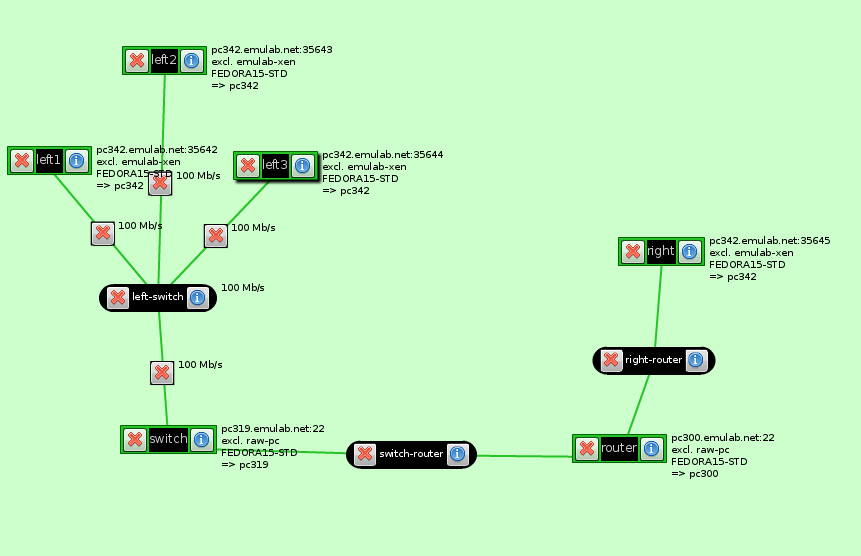
\includegraphics[width=4in]{topology_flack.png}
\end{frame}

\begin{frame}{Demonstration}
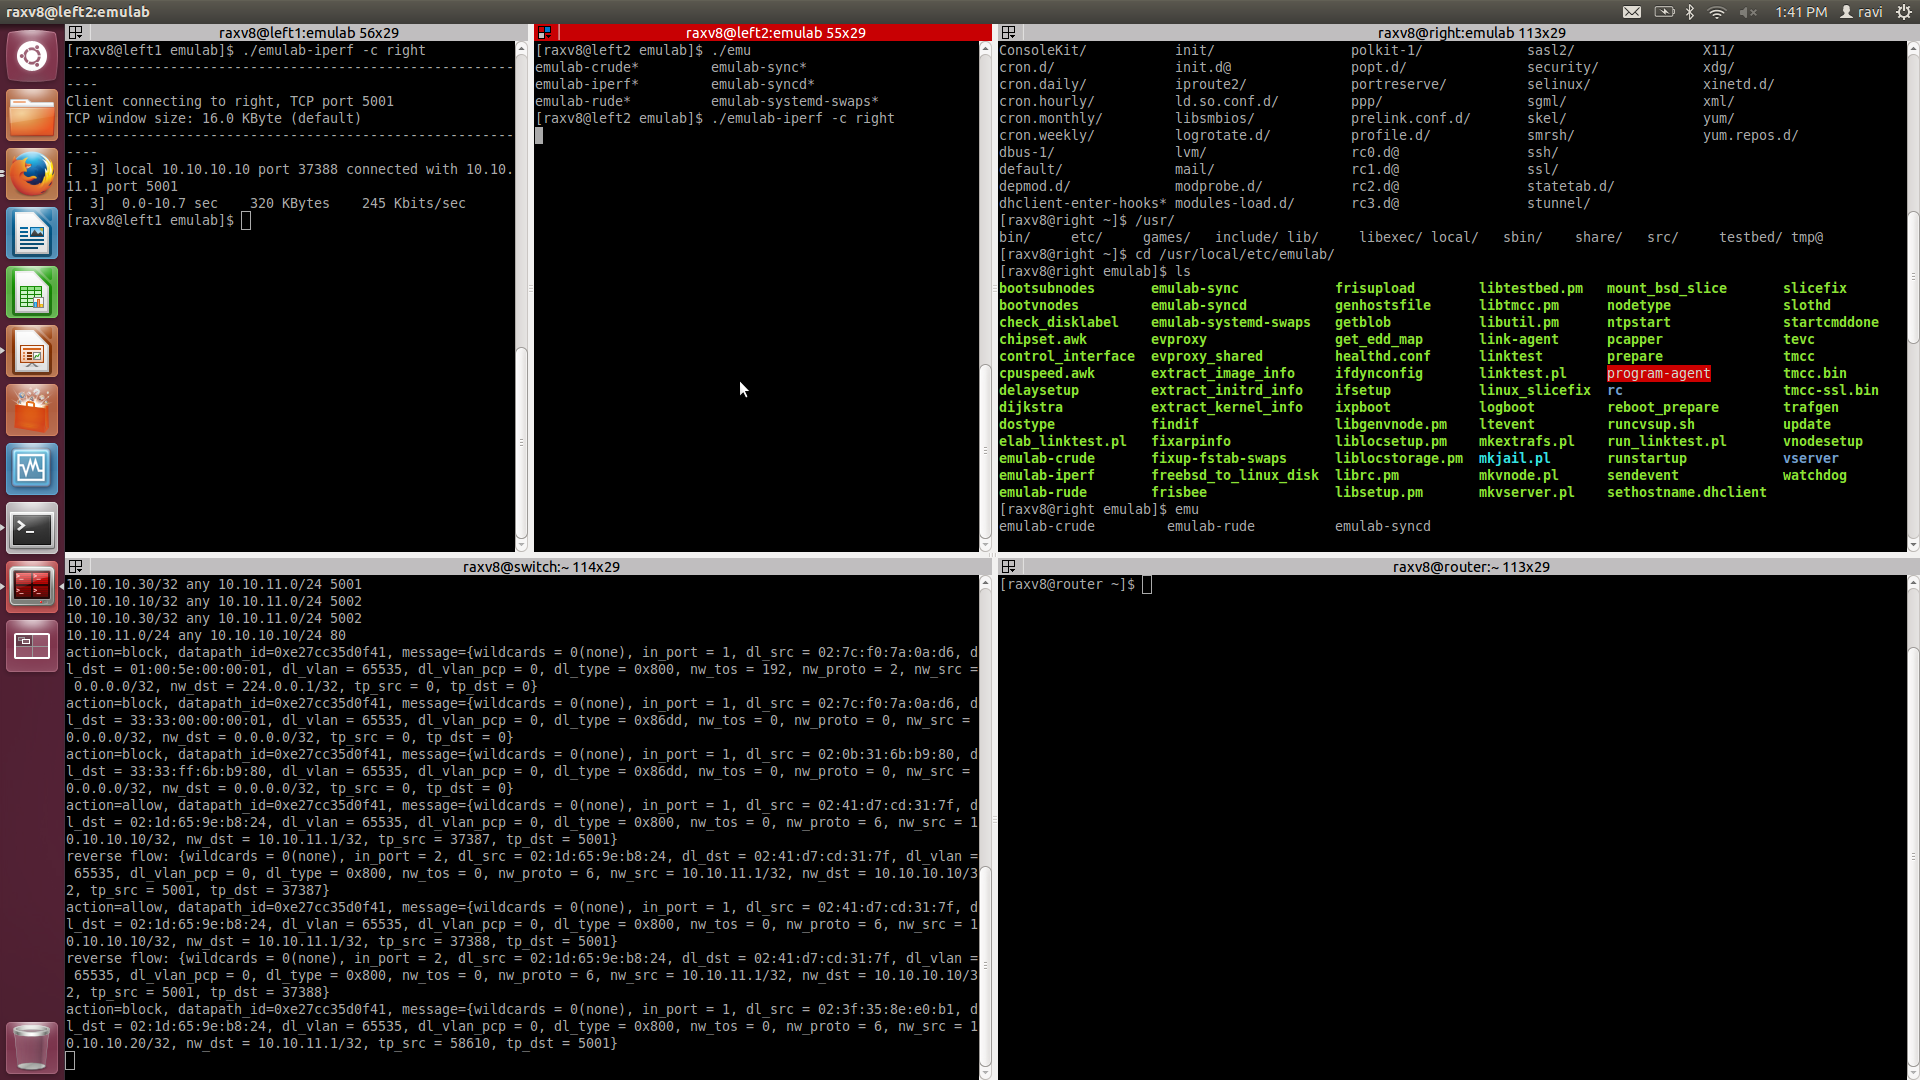
\includegraphics[width=4in]{screenshot.png}
\end{frame}

\begin{frame}{DoS attack detection}
\begin{itemize}
\item We attempted to implement DoS attack detection by SYN floods
\item Lack of time to debug
\end{itemize}
\end{frame}

\begin{frame}{Future work}
\begin{itemize}
\item DoS attack detection (TCP SYN floods)
\item Load balancing or redundancy by multiple paths
\item Repeatable test cases by LabWiki / GIMI
\end{itemize}
\end{frame}

\begin{frame}{Acknowledgements}
\begin{itemize}
\item GPO staff for their support and education
\item GREE camp organising team for their hospitality
\item BBN for hosting the camp
\end{itemize}
\end{frame}

\end{document}
